% Generated by scripts/make_figure.py. Do not edit by hand.
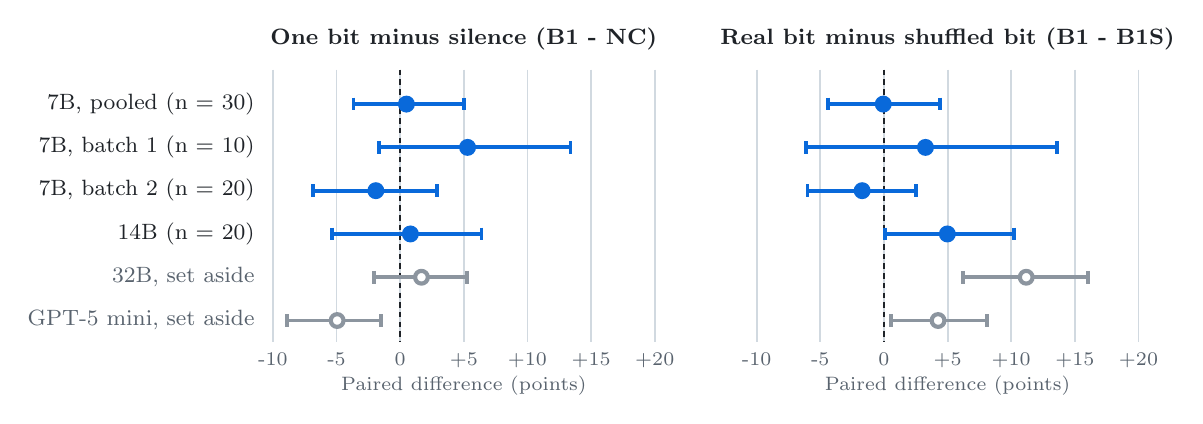
\begin{tikzpicture}
\definecolor{figink}{HTML}{1F2328}
\definecolor{figmuted}{HTML}{59636E}
\definecolor{figgrid}{HTML}{D1D9E0}
\definecolor{figaccent}{HTML}{0969DA}
\definecolor{figsetaside}{HTML}{8C959F}
\definecolor{figwhite}{HTML}{FFFFFF}
\node[anchor=base east, inner sep=0, text=figink, font=\footnotesize] at (85.56pt,107.18pt) {7B, pooled (n = 30)};
\node[anchor=base east, inner sep=0, text=figink, font=\footnotesize] at (85.56pt,91.54pt) {7B, batch 1 (n = 10)};
\node[anchor=base east, inner sep=0, text=figink, font=\footnotesize] at (85.56pt,75.90pt) {7B, batch 2 (n = 20)};
\node[anchor=base east, inner sep=0, text=figink, font=\footnotesize] at (85.56pt,60.26pt) {14B (n = 20)};
\node[anchor=base east, inner sep=0, text=figmuted, font=\footnotesize] at (85.56pt,44.62pt) {32B, set aside};
\node[anchor=base east, inner sep=0, text=figmuted, font=\footnotesize] at (85.56pt,28.98pt) {GPT-5 mini, set aside};
\node[anchor=base, inner sep=0, text=figink, font=\footnotesize\bfseries] at (161.00pt,130.64pt) {One bit minus silence (B1 - NC)};
\draw[figgrid, line width=0.69pt] (92.00pt,121.44pt) -- (92.00pt,23.00pt);
\node[anchor=base, inner sep=0, text=figmuted, font=\scriptsize] at (92.00pt,14.72pt) {-10};
\draw[figgrid, line width=0.69pt] (115.00pt,121.44pt) -- (115.00pt,23.00pt);
\node[anchor=base, inner sep=0, text=figmuted, font=\scriptsize] at (115.00pt,14.72pt) {-5};
\draw[figgrid, line width=0.69pt] (138.00pt,121.44pt) -- (138.00pt,23.00pt);
\node[anchor=base, inner sep=0, text=figmuted, font=\scriptsize] at (138.00pt,14.72pt) {0};
\draw[figgrid, line width=0.69pt] (161.00pt,121.44pt) -- (161.00pt,23.00pt);
\node[anchor=base, inner sep=0, text=figmuted, font=\scriptsize] at (161.00pt,14.72pt) {+5};
\draw[figgrid, line width=0.69pt] (184.00pt,121.44pt) -- (184.00pt,23.00pt);
\node[anchor=base, inner sep=0, text=figmuted, font=\scriptsize] at (184.00pt,14.72pt) {+10};
\draw[figgrid, line width=0.69pt] (207.00pt,121.44pt) -- (207.00pt,23.00pt);
\node[anchor=base, inner sep=0, text=figmuted, font=\scriptsize] at (207.00pt,14.72pt) {+15};
\draw[figgrid, line width=0.69pt] (230.00pt,121.44pt) -- (230.00pt,23.00pt);
\node[anchor=base, inner sep=0, text=figmuted, font=\scriptsize] at (230.00pt,14.72pt) {+20};
\draw[figink, line width=0.69pt, dash pattern=on 2pt off 1.5pt] (138.00pt,121.44pt) -- (138.00pt,23.00pt);
\draw[figaccent, line width=1.38pt] (121.11pt,109.02pt) -- (160.92pt,109.02pt);
\draw[figaccent, line width=1.38pt] (121.11pt,111.32pt) -- (121.11pt,106.72pt);
\draw[figaccent, line width=1.38pt] (160.92pt,111.32pt) -- (160.92pt,106.72pt);
\draw[figaccent, fill=figaccent, line width=1.5pt] (140.26pt,109.02pt) circle (2.30pt);
\draw[figaccent, line width=1.38pt] (130.43pt,93.38pt) -- (199.56pt,93.38pt);
\draw[figaccent, line width=1.38pt] (130.43pt,95.68pt) -- (130.43pt,91.08pt);
\draw[figaccent, line width=1.38pt] (199.56pt,95.68pt) -- (199.56pt,91.08pt);
\draw[figaccent, fill=figaccent, line width=1.5pt] (162.35pt,93.38pt) circle (2.30pt);
\draw[figaccent, line width=1.38pt] (106.49pt,77.74pt) -- (151.38pt,77.74pt);
\draw[figaccent, line width=1.38pt] (106.49pt,80.04pt) -- (106.49pt,75.44pt);
\draw[figaccent, line width=1.38pt] (151.38pt,80.04pt) -- (151.38pt,75.44pt);
\draw[figaccent, fill=figaccent, line width=1.5pt] (129.21pt,77.74pt) circle (2.30pt);
\draw[figaccent, line width=1.38pt] (113.36pt,62.10pt) -- (167.36pt,62.10pt);
\draw[figaccent, line width=1.38pt] (113.36pt,64.40pt) -- (113.36pt,59.80pt);
\draw[figaccent, line width=1.38pt] (167.36pt,64.40pt) -- (167.36pt,59.80pt);
\draw[figaccent, fill=figaccent, line width=1.5pt] (141.70pt,62.10pt) circle (2.30pt);
\draw[figsetaside, line width=1.38pt] (128.44pt,46.46pt) -- (162.13pt,46.46pt);
\draw[figsetaside, line width=1.38pt] (128.44pt,48.76pt) -- (128.44pt,44.16pt);
\draw[figsetaside, line width=1.38pt] (162.13pt,48.76pt) -- (162.13pt,44.16pt);
\draw[figsetaside, fill=figwhite, line width=1.5pt] (145.69pt,46.46pt) circle (2.30pt);
\draw[figsetaside, line width=1.38pt] (97.21pt,30.82pt) -- (131.11pt,30.82pt);
\draw[figsetaside, line width=1.38pt] (97.21pt,33.12pt) -- (97.21pt,28.52pt);
\draw[figsetaside, line width=1.38pt] (131.11pt,33.12pt) -- (131.11pt,28.52pt);
\draw[figsetaside, fill=figwhite, line width=1.5pt] (115.23pt,30.82pt) circle (2.30pt);
\node[anchor=base, inner sep=0, text=figmuted, font=\scriptsize] at (161.00pt,5.52pt) {Paired difference (points)};
\node[anchor=base, inner sep=0, text=figink, font=\footnotesize\bfseries] at (335.80pt,130.64pt) {Real bit minus shuffled bit (B1 - B1S)};
\draw[figgrid, line width=0.69pt] (266.80pt,121.44pt) -- (266.80pt,23.00pt);
\node[anchor=base, inner sep=0, text=figmuted, font=\scriptsize] at (266.80pt,14.72pt) {-10};
\draw[figgrid, line width=0.69pt] (289.80pt,121.44pt) -- (289.80pt,23.00pt);
\node[anchor=base, inner sep=0, text=figmuted, font=\scriptsize] at (289.80pt,14.72pt) {-5};
\draw[figgrid, line width=0.69pt] (312.80pt,121.44pt) -- (312.80pt,23.00pt);
\node[anchor=base, inner sep=0, text=figmuted, font=\scriptsize] at (312.80pt,14.72pt) {0};
\draw[figgrid, line width=0.69pt] (335.80pt,121.44pt) -- (335.80pt,23.00pt);
\node[anchor=base, inner sep=0, text=figmuted, font=\scriptsize] at (335.80pt,14.72pt) {+5};
\draw[figgrid, line width=0.69pt] (358.80pt,121.44pt) -- (358.80pt,23.00pt);
\node[anchor=base, inner sep=0, text=figmuted, font=\scriptsize] at (358.80pt,14.72pt) {+10};
\draw[figgrid, line width=0.69pt] (381.80pt,121.44pt) -- (381.80pt,23.00pt);
\node[anchor=base, inner sep=0, text=figmuted, font=\scriptsize] at (381.80pt,14.72pt) {+15};
\draw[figgrid, line width=0.69pt] (404.80pt,121.44pt) -- (404.80pt,23.00pt);
\node[anchor=base, inner sep=0, text=figmuted, font=\scriptsize] at (404.80pt,14.72pt) {+20};
\draw[figink, line width=0.69pt, dash pattern=on 2pt off 1.5pt] (312.80pt,121.44pt) -- (312.80pt,23.00pt);
\draw[figaccent, line width=1.38pt] (292.61pt,109.02pt) -- (333.11pt,109.02pt);
\draw[figaccent, line width=1.38pt] (292.61pt,111.32pt) -- (292.61pt,106.72pt);
\draw[figaccent, line width=1.38pt] (333.11pt,111.32pt) -- (333.11pt,106.72pt);
\draw[figaccent, fill=figaccent, line width=1.5pt] (312.56pt,109.02pt) circle (2.30pt);
\draw[figaccent, line width=1.38pt] (284.51pt,93.38pt) -- (375.42pt,93.38pt);
\draw[figaccent, line width=1.38pt] (284.51pt,95.68pt) -- (284.51pt,91.08pt);
\draw[figaccent, line width=1.38pt] (375.42pt,95.68pt) -- (375.42pt,91.08pt);
\draw[figaccent, fill=figaccent, line width=1.5pt] (327.82pt,93.38pt) circle (2.30pt);
\draw[figaccent, line width=1.38pt] (285.20pt,77.74pt) -- (324.43pt,77.74pt);
\draw[figaccent, line width=1.38pt] (285.20pt,80.04pt) -- (285.20pt,75.44pt);
\draw[figaccent, line width=1.38pt] (324.43pt,80.04pt) -- (324.43pt,75.44pt);
\draw[figaccent, fill=figaccent, line width=1.5pt] (304.93pt,77.74pt) circle (2.30pt);
\draw[figaccent, line width=1.38pt] (313.07pt,62.10pt) -- (359.83pt,62.10pt);
\draw[figaccent, line width=1.38pt] (313.07pt,64.40pt) -- (313.07pt,59.80pt);
\draw[figaccent, line width=1.38pt] (359.83pt,64.40pt) -- (359.83pt,59.80pt);
\draw[figaccent, fill=figaccent, line width=1.5pt] (335.72pt,62.10pt) circle (2.30pt);
\draw[figsetaside, line width=1.38pt] (341.46pt,46.46pt) -- (386.42pt,46.46pt);
\draw[figsetaside, line width=1.38pt] (341.46pt,48.76pt) -- (341.46pt,44.16pt);
\draw[figsetaside, line width=1.38pt] (386.42pt,48.76pt) -- (386.42pt,44.16pt);
\draw[figsetaside, fill=figwhite, line width=1.5pt] (364.22pt,46.46pt) circle (2.30pt);
\draw[figsetaside, line width=1.38pt] (315.44pt,30.82pt) -- (350.15pt,30.82pt);
\draw[figsetaside, line width=1.38pt] (315.44pt,33.12pt) -- (315.44pt,28.52pt);
\draw[figsetaside, line width=1.38pt] (350.15pt,33.12pt) -- (350.15pt,28.52pt);
\draw[figsetaside, fill=figwhite, line width=1.5pt] (332.37pt,30.82pt) circle (2.30pt);
\node[anchor=base, inner sep=0, text=figmuted, font=\scriptsize] at (335.80pt,5.52pt) {Paired difference (points)};
\end{tikzpicture}
